\documentclass{beamer}

\usepackage[utf8]{inputenc}
\usepackage[T1]{fontenc}
\usepackage{amsmath}
\usepackage{bm}

\usepackage{tabularx}
\usepackage{graphicx}
\usepackage{epstopdf}
\usepackage{multirow}

\graphicspath{{../../images/}}

\usetheme{Madrid}
\usebeamercolor{sidebartab}
\usefonttheme{professionalfonts}


\title[M.Sc. Thesis 2015]{Spatial Summarization of Image Collections}
\author{Diego A. Ballesteros Villamizar}
\institute[ETHZ]{ETH Zürich}
\date{March 18th, 2016}

\DeclareMathOperator*{\argmin}{argmin}
\DeclareMathOperator*{\argmax}{argmax}

\AtBeginSection[]
{
  \begin{frame}<beamer>
    \frametitle{Outline}
    \tableofcontents[currentsection]
  \end{frame}
}

\begin{document}

\begin{frame}
  \titlepage
\end{frame}

\section{Synthetic Featurized Data}

\begin{frame}{Featurized model}
  \begin{itemize}
    \item $|V| = 7$
    \item \begin{equation*}
      \mathbf{X} = \left( \begin{array}{ccc}
      5 & 0 & 1 \\
      5 & 1 & 0 \\
      5 & 1 & 1 \\
      3 & 0 & 1 \\
      3 & 0 & 0 \\
      1 & 1 & 1 \\
      1 & 1 & 0 \end{array} \right)
    \end{equation*}
    \item $\mathbf{a} = \overrightarrow{0}$
    \item $\mathbf{B} = \left( \begin{array}{ccc} 0 & 20 & 20\end{array}\right)^{\intercal}$
    \item $\mathbf{C} = \left( \begin{array}{ccc} 2 & 0 & 0 \end{array}\right)^{\intercal}$
  \end{itemize}
\end{frame}

\begin{frame}{FLDC equivalent model}
  \begin{itemize}
    \item $\mathbf{u} = \overrightarrow{0}$
    \item $\mathbf{W}_{D} = \left( \begin{array}{ccccccc} 20 & 20 & 40 & 20 & 0 & 40 & 20 \end{array}\right)^{\intercal}$
    \item $\mathbf{W}_{C} = \left( \begin{array}{ccccccc} 10 & 10 & 10 & 6 & 6 & 2 & 2 \end{array}\right)^{\intercal}$
    \item $P(S) \approx 0.25 \mid S \in \{\{0, 4\}, \{1, 4\}, \{2, 4\}, \{3, 4\}\}$
  \end{itemize}
\end{frame}

\begin{frame}{Learning results}
  \begin{itemize}
    \item 10,000 samples from the distribution.
    \item The maximum prediction accuracy is $62.5\%$.
    \item After 10 passes:
      \begin{itemize}
        \item $\mathbf{a} = \left( \begin{array}{ccc} 0.05 \pm 0.03 & -0.37 \pm 0.03 & -0.31 \pm 0.03 \end{array} \right)$
        \item $\mathbf{B} = \left( \begin{array}{ccc} 0.81 \pm 0.03 & 8.33 \pm 0.02 & 8.33 \pm 0.02 \end{array}\right)^{\intercal}$
        \item $\mathbf{C} = \left( \begin{array}{ccc} 1.82 \pm 0.01 & 0.00 \pm 0.00 & 0.00 \pm 0.00 \end{array}\right)^{\intercal}$
      \end{itemize}
    \item After 50 passes:
      \begin{itemize}
        \item $\mathbf{a} = \left( \begin{array}{ccc} 0.01 \pm 0.03 & -0.05 \pm 0.04 & -0.03 \pm 0.03 \end{array} \right)$
        \item $\mathbf{B} = \left( \begin{array}{ccc} 0.60 \pm 0.03 & 12.5 \pm 0.03 & 12.5 \pm 0.03 \end{array}\right)^{\intercal}$
        \item $\mathbf{C} = \left( \begin{array}{ccc} 2.11 \pm 0.03 & 0.00 \pm 0.00 & 0.00 \pm 0.00 \end{array}\right)^{\intercal}$
      \end{itemize}
  \end{itemize}
\end{frame}

\begin{frame}{NCE objective}
  \begin{figure}
    \centering
    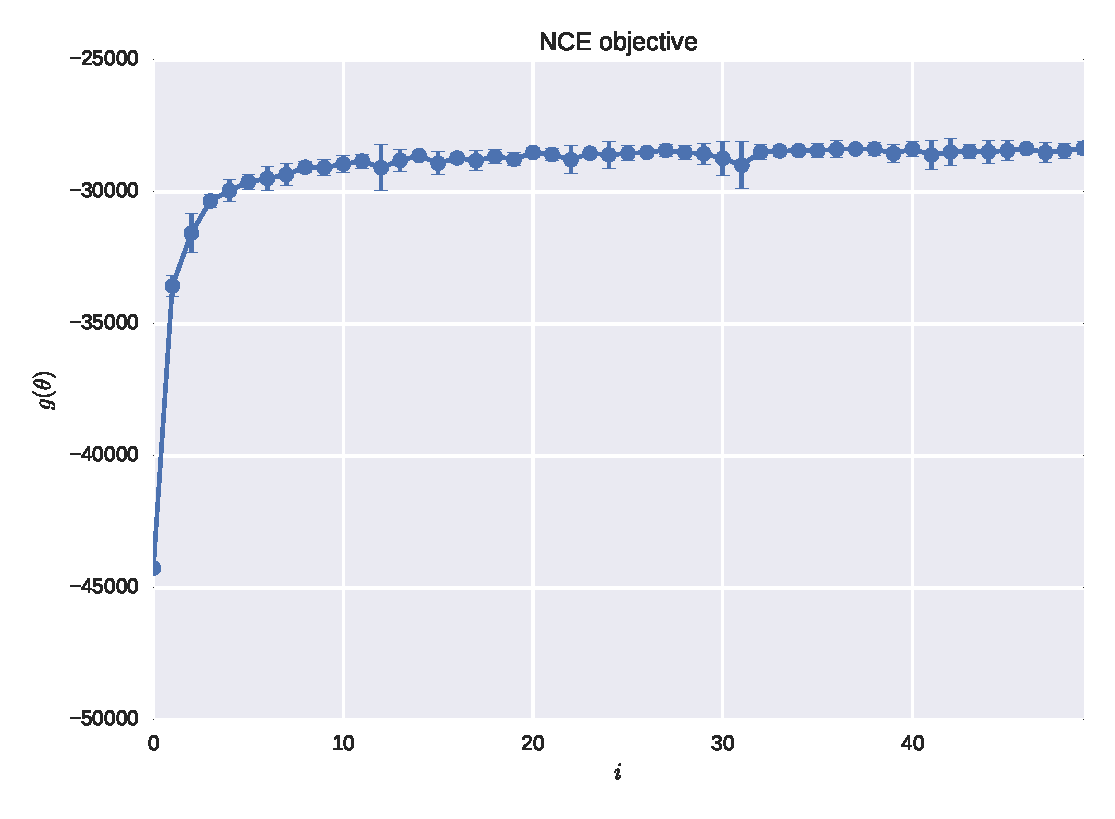
\includegraphics[height=0.8\textheight]{synthetic_3_objective}
  \end{figure}
\end{frame}

\begin{frame}{Featurized model II}
  \begin{itemize}
    \item \begin{equation*}
      \mathbf{X} = \left( \begin{array}{ccc}
      5 & 0 & 1 \\
      4 & 1 & 0 \\
      4 & 1 & 1 \\
      3 & 0 & 1 \\
      3 & 1 & 0 \\
      2 & 1 & 1 \\
      2 & 1 & 0 \end{array} \right)
    \end{equation*}
    \item \begin{equation*}
      \mathbf{B} = \left( \begin{array}{cc}
      0 & 0 \\
      10 & 0 \\
      0 & 10 \end{array} \right)
    \end{equation*}
    \item $\mathbf{C} = \left( \begin{array}{ccc} 1 & 0 & 0 \end{array}\right)^{\intercal}$
  \end{itemize}
\end{frame}

\begin{frame}{FLDC equivalent model}
  \begin{itemize}
   \item \begin{equation*}
     \mathbf{W}_{D} = \left( \begin{array}{cc}
     0 & 10 \\
     10 & 0 \\
     10 & 10 \\
     0 & 10 \\
     10 & 0 \\
     10 & 10 \\
     10 & 0 \end{array} \right)
   \end{equation*}
    \item $\mathbf{W}_{C} = \left( \begin{array}{ccccccc} 5 & 4 & 4 & 3 & 3 & 2 & 2 \end{array}\right)^{\intercal}$
    \item $P(\{0,1\}) \approx 0.4$
    \item $P(S) \approx 0.15 \mid S \in \{\{1,3\}, \{0,4\}, \{3,4\}\}$
    \item $P(S) \approx 0.05 \mid S \in \{\{0,6\}, \{3,6\}\}$
  \end{itemize}
\end{frame}

\begin{frame}{Learning results}
  \begin{itemize}
    \item 100 pass over data and noise.
    \item $\mathbf{u} = \left( \begin{array}{ccc} 0.19 & 0.22 & 0.14 \end{array}\right)^{\intercal}$
    \item \begin{equation*}
      \mathbf{B} = \left( \begin{array}{cc}
      0.27 & 0.25 \\
      0.07 & 9.66 \\
      9.46 & 0.08 \end{array} \right)
    \end{equation*}
    \item $\mathbf{C} = \left( \begin{array}{ccc} 1.11 & 0.84 & 0.80 \end{array}\right)^{\intercal}$
  \end{itemize}
\end{frame}

\begin{frame}{Learning results - FLDC}
  \begin{itemize}
    \item $\mathbf{u} = \left( \begin{array}{ccccccc} 0.69 & 0.48 & -4.58 & 0.12 & -0.22 & -4.30 & -1.09 \end{array}\right)^{\intercal}$
    \item \begin{equation*}
      \mathbf{W}_{D} = \left( \begin{array}{cc}
      0.81 & 3.66 \\
      3.93 & 0.81 \\
      0.95 & 0.98 \\
      0.80 & 3.66 \\
      3.40 & 0.74 \\
      1.04 & 0.94 \\
      3.41 & 0.67 \end{array} \right)
    \end{equation*}
    \item $\mathbf{W}_{C} = \left( \begin{array}{ccccccc} 1.71 & 1.71 & 0.38 & 1.73 & 1.72 & 0.24 & 1.44 \end{array}\right)^{\intercal}$
  \end{itemize}
\end{frame}

\begin{frame}{Learned models}
  \begin{table}
    \centering
    \begin{tabular}{@{}lllll@{}}
      \hline
      \textbf{Subset} & \textbf{Model} & \textbf{Modular} & \textbf{FLDC} & \textbf{FFLDC} \\
      \hline
      $\{0,1\}$ & $0.40$ & $0.14 \pm 0.00$ & $0.29 \pm 0.05$ & $0.36 \pm 0.05$  \\
      $\{0,4\}$ & $0.15$ & $0.04 \pm 0.00$ & $0.10 \pm 0.03$ & $0.11 \pm 0.03$ \\
      $\{1,3\}$ & $0.15$ & $0.05 \pm 0.00$ & $0.12 \pm 0.04$ & $0.12 \pm 0.03$ \\
      $\{3,4\}$ & $0.15$ & $0.02 \pm 0.00$ & $0.09 \pm 0.03$ & $0.13 \pm 0.04$ \\
      $\{0,6\}$ & $0.05$ & $0.02 \pm 0.00$ & $0.04 \pm 0.01$ & $0.03 \pm 0.01$ \\
      $\{3,6\}$ & $0.05$ & $0.00 \pm 0.00$ & $0.03 \pm 0.01$ & $0.05 \pm 0.02$ \\
      \hline
    \end{tabular}
  \end{table}
\end{frame}

\section{Featurized Learning}

\begin{frame}{Larger dataset}
  \begin{itemize}
    \item Increase the number of selected clusters to 100.
    \item The best results without features are:
  \end{itemize}
  \begin{figure}
    \centering
    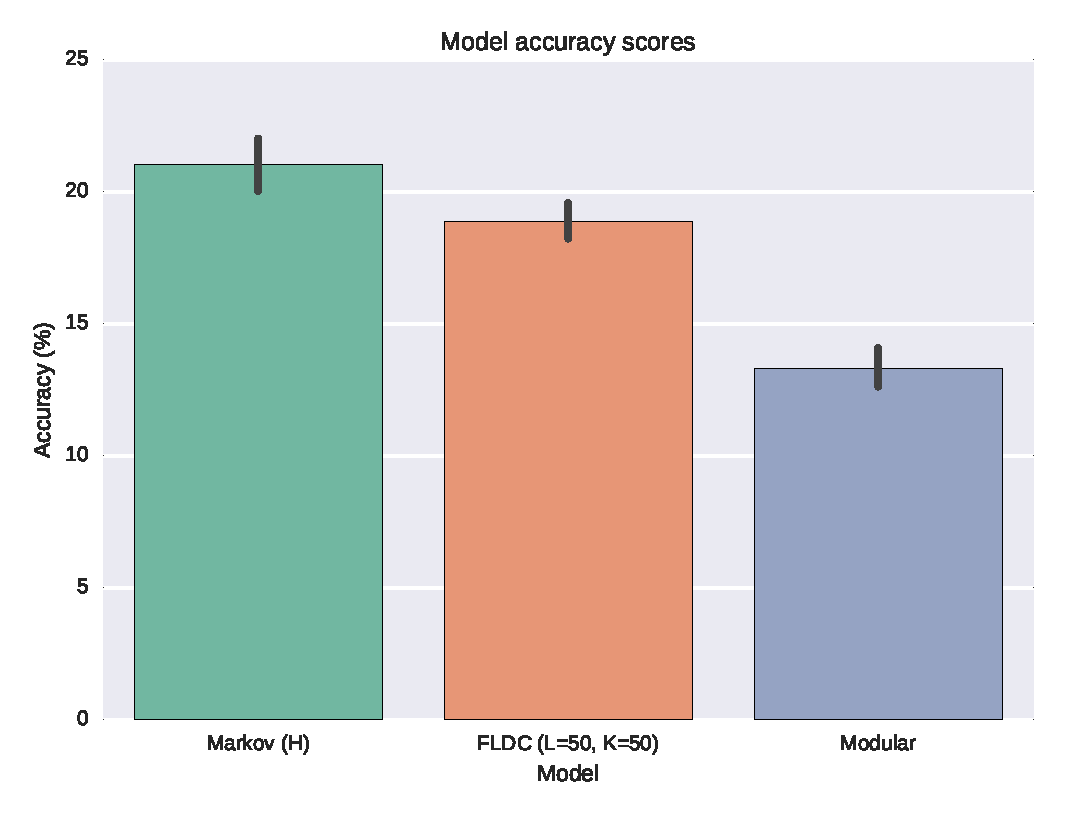
\includegraphics[height=0.5\textheight]{score_100_no_singles_no_features}
  \end{figure}
\end{frame}

\begin{frame}{FLDC model}
  \begin{figure}
    \centering
    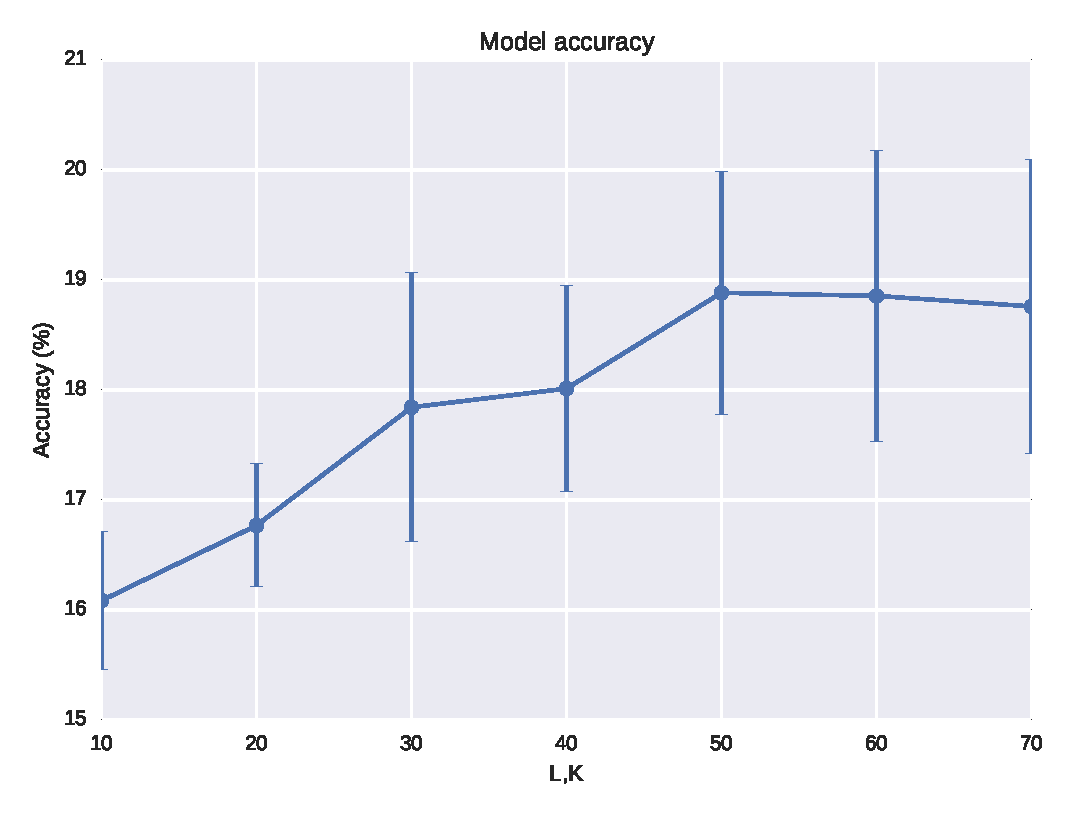
\includegraphics[height=0.8\textheight]{score_100_no_singles_no_features_dim}
  \end{figure}
\end{frame}

\begin{frame}{Selecting the features}
  \begin{itemize}
    \item If $\sigma$ is too big then the feature matrix is full of 1s.
    \item If $\sigma$ is too small then the feature matrix is too similar to the identity.
  \end{itemize}
  \begin{figure}
    \centering
    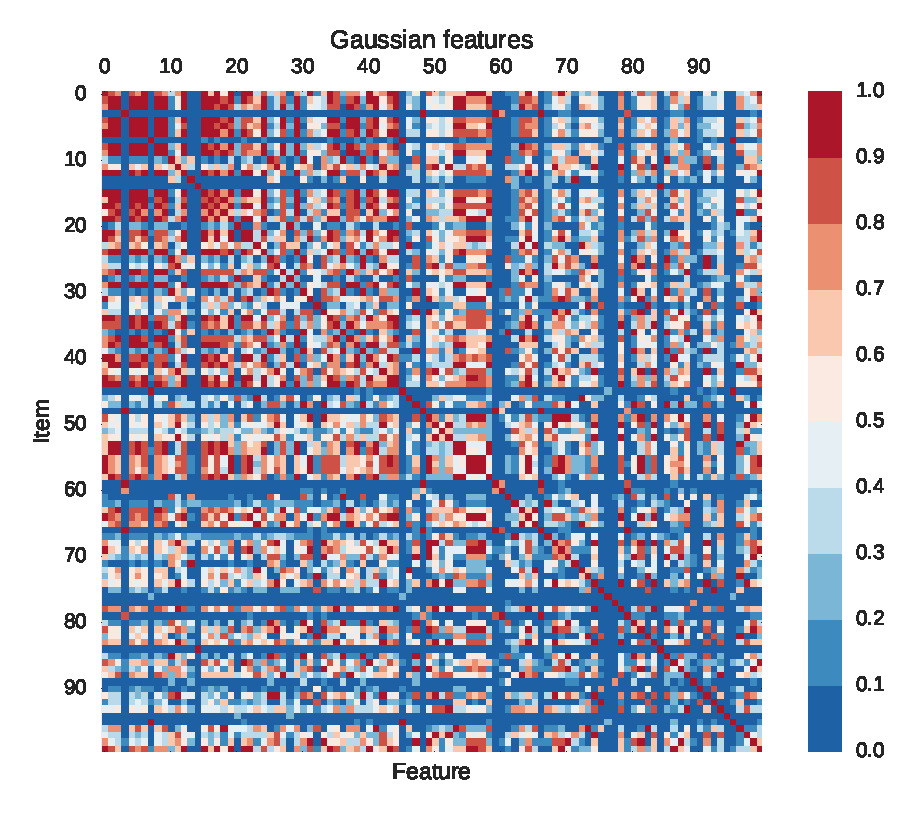
\includegraphics[height=0.5\textheight]{gaussian_features_n_100_0dot15}
  \end{figure}
\end{frame}

\begin{frame}{Using 10 features}
  \begin{figure}
    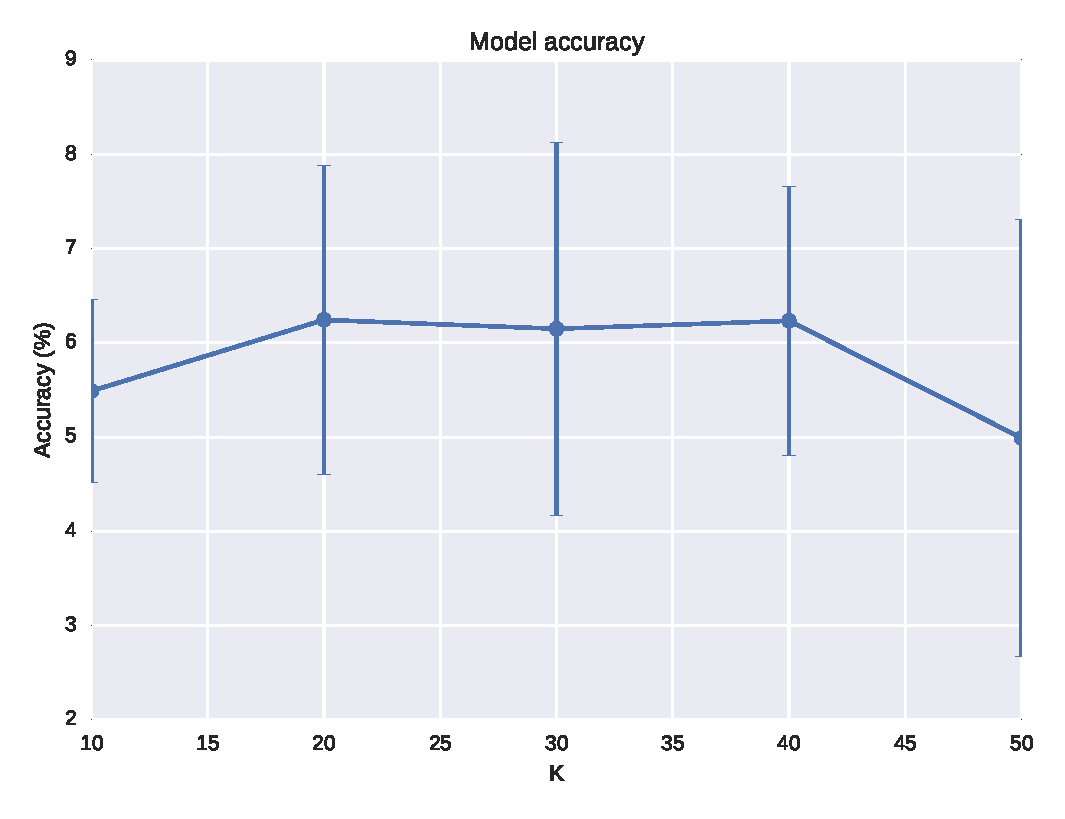
\includegraphics[height=0.8\textheight]{score_100_no_singles_features_only_coherence}
  \end{figure}
\end{frame}

\begin{frame}{Best results}
  \begin{figure}
    \centering
    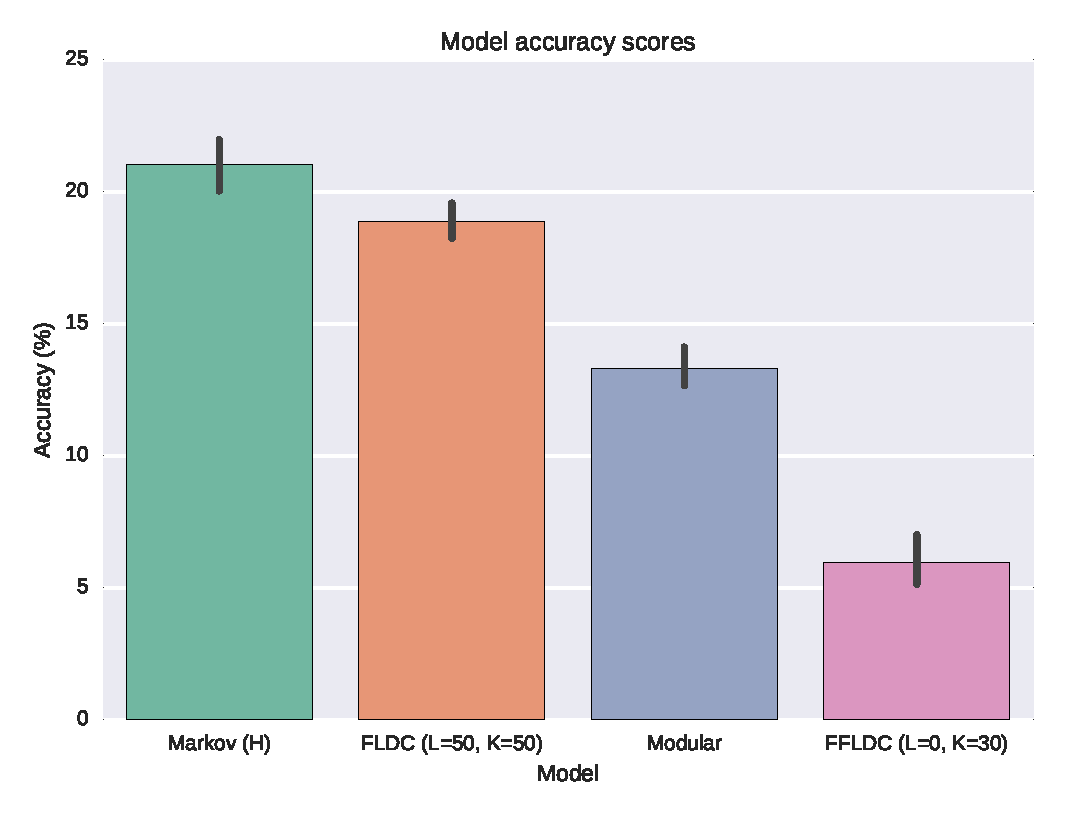
\includegraphics[height=0.8\textheight]{score_100_no_singles_with_features}
  \end{figure}
\end{frame}

\begin{frame}{NCE Learning}
  \begin{figure}
    \centering
    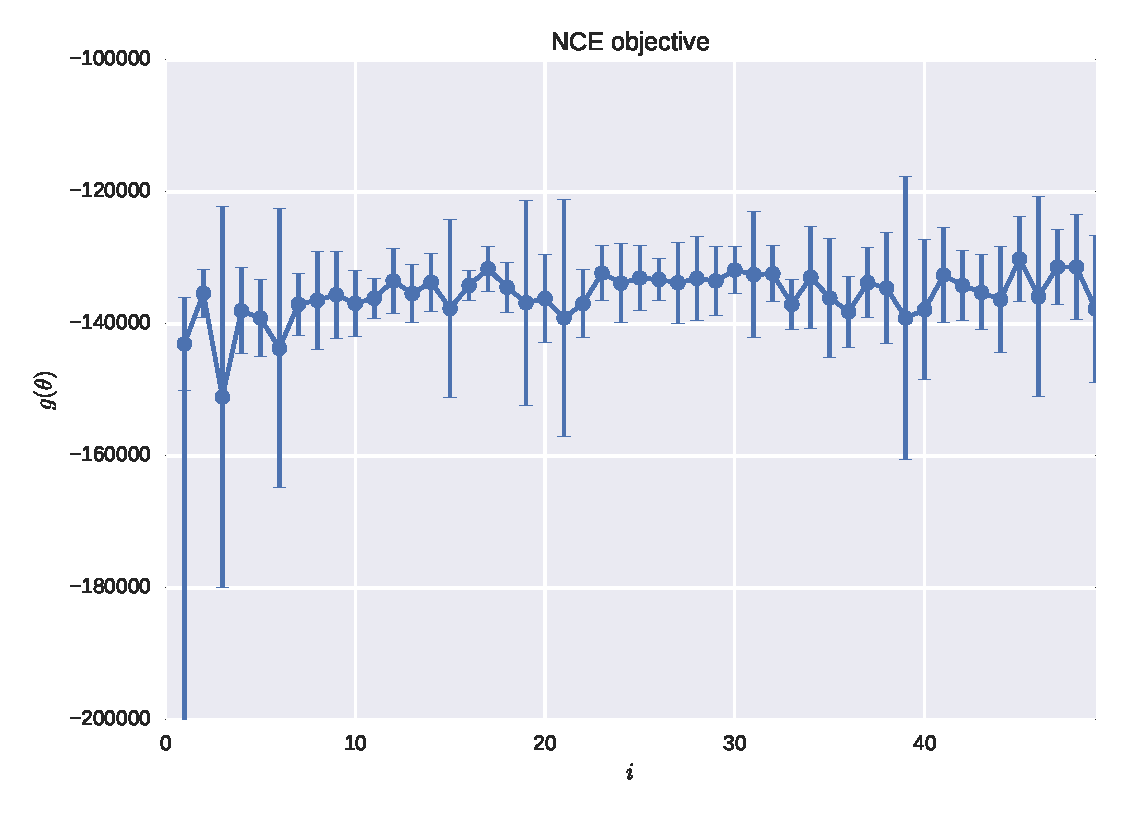
\includegraphics[height=0.8\textheight]{100_no_singles_features_objective}
  \end{figure}
\end{frame}

\section{Document outline}

\begin{frame}[allowframebreaks]{Outline}
  \begin{enumerate}
    \item Introduction
      \begin{enumerate}
        \item Motivation
        \item Related work
      \end{enumerate}
    \item Theoretical framework
      \begin{enumerate}
        \item Clustering - Mean-shift
        \item Probabilistic Submodular Models
        \item NCE learning
      \end{enumerate}
    \item Datasets
      \begin{enumerate}
        \item Image collections
          \begin{enumerate}
            \item Dataset crawling \& Flickr
            \item Zürich dataset
          \end{enumerate}
        \item Clustering and paths
          \begin{enumerate}
            \item Clustering and filtering
            \item Path identification
          \end{enumerate}
       \end{enumerate}
    \item Models and learning
      \begin{enumerate}
        \item FLID - Submodular only
        \item FLDC - Submodular and supermodular components
        \item FFLDC - FLDC with features
      \end{enumerate}
    \item Results \& Discussion
      \begin{enumerate}
        \item Baseline models
        \item 10 items
        \item 100 items
      \end{enumerate}
    \item Conclusion
  \end{enumerate}
\end{frame}
%\begin{frame}{References}
%  \bibliographystyle{acm}
%  \bibliography{../references}
%\end{frame}

\end{document}
